\chapter{TECNOLOGIAS}
\label{cap:conclusao}

Durante o estágio, tive a possibilidade de testar e utilizar diversas tecnologias e frameworks.
Para melhor entendimento do trabalho, é necessário um dissertação sobre as mesmas.

\section{Frontend}

Os Frameworks pricipais de frontend são ReactJs, Angular e Vuejs.
Sendo ReactJS e VueJs os principais em favoritos dentro da comunidade do GitHub

\begin{figure}[H]
\centering
\caption{Comparação frameworks frotnend pelo github} %legenda
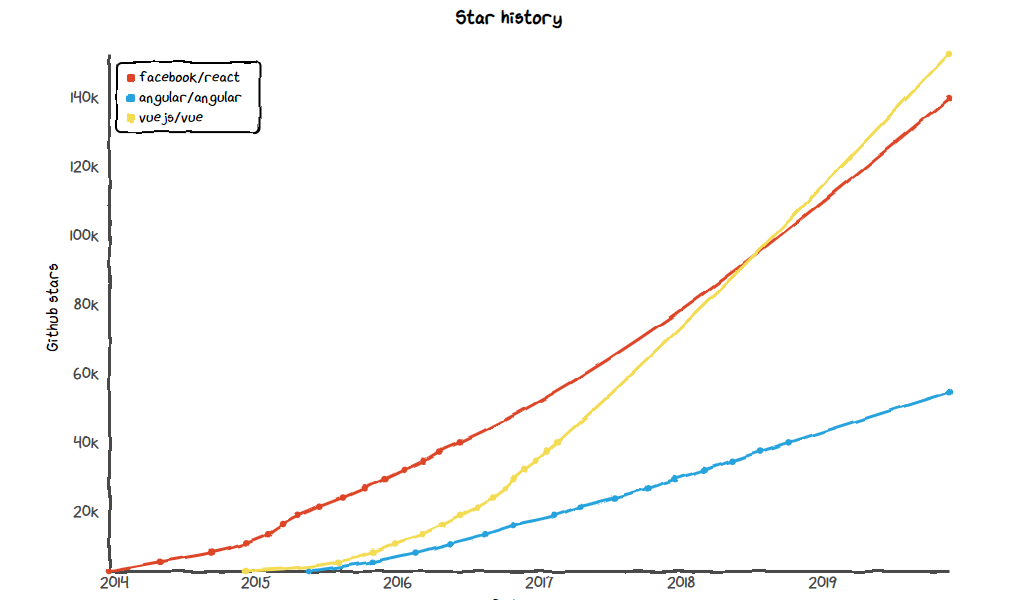
\includegraphics[scale=0.35]{githubFramework}\\  % o 0.9 indica 90% do tamanho original
\label{fig:exemplo} %rotulo para refencia
{\small Fonte: https://star-history.t9t.io} %Fonte da imagem
\end{figure}

Com seu lançamento tardio em relação ao reactjs, o vuejs vem crescendo e neste ano de 2019 ultrapassou o numero de estrelas no github, enquanto o framework angular
 cresce de forma lenta e continua.

Os frameworks VueJs e ReactJs tinham como grande diferencial o uso da Virtual DOM em vez da DOM(Document Object Model). Uma vez que a DOM era uma abstração do codigo HTML, a DOM Virtual é uma abstração da DOM.

Enquanto a DOM é uma arvore de objetos interligados, com diversas conexões e ramificações, onde modificações simples nos mesmos eram muito frequentes. Já a DOM virtual veio para 
solucionar este problema, ela já possui configurações e implementações do browser, livrando o desenvolvedor de ter que configura-las manualmente. Alem disto a DOM virtual é mais leve e simples, sendo mais facil compreende-la e desenvolve-la.

Outro grande diferencial graças a esta mudança, é que a abstração de componentes se tornou mais inteligente, uma vez que era possível desenvolver componentes desacoplados e acoplados somente onde eram necessários.

No inicio do estágio, diversos projetos que tive contato eram utilizado angular, por conta de ter sido lançado em 2010 pela Google. Foi uma grande evolução, uma vez que projetos mais velhos foram desenvolvidos em Flex, que era uma tecnologia para interfaces em flash com integração com java.

O framework angular facilitava absurdamente o trabalho como desenvolvedor, uma vez que em diversos casos, que seriam necessárias diversas linhas de Jquery e Javascript, erá somente nescessario o uso de uma.


\begin{figure}[!htb]
\centering
\caption{Adicionando evento a elementos DOM pelo JQuery} %legenda
\begin{lstlisting}
var box = $( "#box" );
$( "#botao" ).on( "click", function( event ) {
    box.show();
});
\end{lstlisting} 
\label{fig:exemplocodigo1} %rotulo para refencia
\end{figure}

\begin{figure}[!htb]
\centering
\caption{Adicionando evento a elementos VirtualDOM pelo Angular} %legenda
\begin{lstlisting}
<div ng-show={show} ng-click={() => {show = true}}/>
\end{lstlisting} 
\label{fig:exemplocodigo1} %rotulo para refencia
\end{figure}
    

Como a base de desenvolvedores no LEMAF já possuia muita experiencia com Angular, foi difícil fazer com que adotassem outras tecnologias em outros projetos.

Porém logo apos iniciativa de um desenvolvedor de um time, apresentamos o VueJs para a organização do LEMAF e conseguimos com que os projetos fossem desenvolvidos com ele.

O VueJs não possuia documentação vasta como o do Angular, porem possuia atualizações recorrentes, porem com sua acensão, foi fácil demonstrar que em alguns anos a documentação dele seria melhor que a do angular.

Porém era complicado mesmo assim, pois a credibilidade de um framework da Google contra a de um ex-desenvolvedor da Google(Criador do VueJs) era incomparável, era realmente um risco a mudança. 
Mas ao mostrar que o projeto recebia uma grande verba de patrocínio, a curva de crescimento e que o mesmo possuia uma equipe fixa de pelo menos 50 contribuidores, entenderam que o risco não era tão grande.

A adesão ao Vue foi muito bem aceita em diversas equipes, pois a flexibilidade que ele proporciona ao desenvolvedor comparado ao angular era gigantesca, com a possibilidade de configuração quase infinita, diversas bibliotecas e varios modos de arquitetura, o vue se tornou foco de estudo na empresa.
Uma das iniciativas vindas dos organizadores da empresa foi fornecer alguns cursos da plataforma Alura para desenvolvimento web com VueJs.

Sua performance mesmo com sendo maior que o ReactJS demonstrava mais fluidez, desde a ferramente de hot-reload até a compilação para modo produção.
Sua arquitetura era simples e direta, centralizada em poucos arquivos e ao mesmo tempo separava bem os comportamentos. Sua documentação era bem escrita, descrevendo os ciclos de vida dos componentes até suas diretivas.

Muitos aprenderam por conta própria facilmente, uma vez que a complexidade abaixava, tendo toda a estrutura de um componente do angular com 5 arquivos, em 1 arquivo .vue somente.
Como vários módulos do LEMAF já utilizavam de Pug/Jade em vez do HTML puro, a transição foi muito tranquila, pois vue já suportava Pug e diversas outras linguagens.

Outro beneficio grande encontrado durante a transição foram as bibliotecas de UI, pois com angular o mais adequado era o uso do Material Design que já era da própria empresa ou 
bootstrap, porém com o VueJs vieram varias outras bibliotecas como Vuetify e ElementUI, que tornaram as interfaces bem mais leves, modernas e bonitas, saindo daquele estilo antigo e estático.

Também foi apresentado para a organização neste estagio a ideia de Design System, que era algo que seria fácil de ser aplicado graças ao VueJs, que componentização facilmente os componentes e que se usado 
de forma correta(Separando componentes de visualização e logica), poderia melhorar significantemente o tempo para desenvolvimento dos projetos.

Em 2019, vendo o advento das tecnologias de desenvolvimento hibrido para mobile, foi questionado a nos se seria interessante o uso de frameworks mais próximos, para possíveis futuros projetos.
Dai a adesão ao ReactJs, já que o principal utilizado para desenvolvimento mobile era o react-native, que se assemelhava bastante.

Ao estudarmos sobre, entendemos que a curva de aprendizado para quem desenvolvia Vue iria ser bem pequena, já que ambos eram bem flexíveis.

Ele era mais leve que o vue que já era muito leve e ainda possuia uma documentação muito boa.
Porem um grande diferencial que existia era o uso do JSX, uma versão do Javascript que combina elementos do HTML dentro do Javascript. Era bem legível e bem similar ao HTML, mas não tinha um bom suporte para Pug.

Mesmo com este problema, resolvemos testar um projeto pequeno com ele. 

As primeiras semanas foram difíceis, tivemos que estudar muito sobre o framework pois ele possuia diversas bibliotecas que melhoravam significantemente seu uso.

Apos as duas primeiras semanas o desenvolvimento fluiu, as duvidas eram pouco recorrentes e as respostas eram fáceis de encontrar. Porem voltamos ao problema inicial do angular, 
a falta de um biblioteca de UI que combinasse com a identidade da empresa.

Foi colocado então em pratica a construção do Design System, um processo de construção de identidade visual para empresa, com componentes próprios desenvolvidos com excelência para poderem ser utilizados em varios projetos, facilitando o desenvolvimento de todos e garantindo qualidade.

A criação dessa biblioteca tinha como objetivo fazer com que os desenvolvedores centralizassem os componentes, contribuindo publicamente com a biblioteca, sendo mais fácil corrigir um erro e depois atualizar a biblioteca que resolve-lo em todos projetos.

E isto se tornou prazeroso com ReactJS, pois o suporte para componentização por ele é ótimo, desde o desenvolvimento até a criação dos testes automatizados.
